\section{Demo}

\begin{frame}{}
  \begin{center}
    \Large{Demonstration}
  \end{center}
\end{frame}


\begin{frame}{\texttt{MSnSet} data structure}

  \begin{figure}[h]
    \centering
    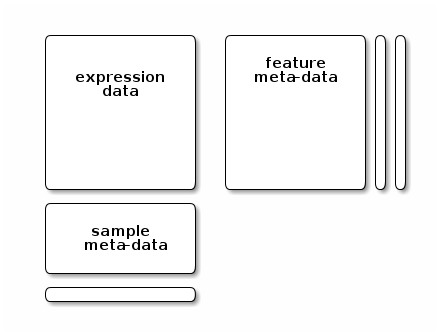
\includegraphics[width=.8\linewidth]{./figs/msnset.png}
    \label{fig:msnset}
  \end{figure}

\end{frame}


\begin{frame}[fragile]
\begin{knitrout}
\definecolor{shadecolor}{rgb}{0.969, 0.969, 0.969}\color{fgcolor}\begin{kframe}
\begin{alltt}
\hlkwd{library}\hlstd{(}\hlstr{"pRoloc"}\hlstd{)}
\hlkwd{library}\hlstd{(}\hlstr{"pRolocdata"}\hlstd{)}
\hlkwd{data}\hlstd{(hyperLOPIT2015)}

\hlkwd{setStockcol}\hlstd{(}\hlkwd{paste0}\hlstd{(}\hlkwd{getStockcol}\hlstd{(),} \hlnum{80}\hlstd{))}

\hlkwd{library}\hlstd{(}\hlstr{"magrittr"}\hlstd{)}
\hlkwd{library}\hlstd{(}\hlstr{"dplyr"}\hlstd{)}
\hlkwd{library}\hlstd{(}\hlstr{"ggplot2"}\hlstd{)}
\end{alltt}
\end{kframe}
\end{knitrout}
\end{frame}

\begin{frame}[fragile]
\begin{knitrout}
\definecolor{shadecolor}{rgb}{0.969, 0.969, 0.969}\color{fgcolor}\begin{kframe}
\begin{alltt}
\hlkwd{plot2D}\hlstd{(hyperLOPIT2015,} \hlkwc{fcol} \hlstd{=} \hlkwa{NULL}\hlstd{,}
       \hlkwc{col} \hlstd{=} \hlstr{"#00000025"}\hlstd{,} \hlkwc{pch} \hlstd{=} \hlnum{19}\hlstd{)}
\hlkwd{plot2D}\hlstd{(hyperLOPIT2015,} \hlkwc{method} \hlstd{=} \hlstr{"hexbin"}\hlstd{)}
\hlkwd{plot2D}\hlstd{(hyperLOPIT2015)}

\hlkwd{plot2D}\hlstd{(hyperLOPIT2015,} \hlkwc{fcol} \hlstd{=} \hlstr{"final.assignment"}\hlstd{)}
\hlstd{sz} \hlkwb{<-} \hlkwd{exp}\hlstd{(}\hlkwd{fData}\hlstd{(hyperLOPIT2015)}\hlopt{$}\hlstd{svm.score)} \hlopt{-} \hlnum{1}
\hlkwd{plot2D}\hlstd{(hyperLOPIT2015,} \hlkwc{fcol} \hlstd{=} \hlstr{"final.assignment"}\hlstd{,}
       \hlkwc{cex} \hlstd{= sz)}
\hlkwd{addLegend}\hlstd{(hyperLOPIT2015)}
\end{alltt}
\end{kframe}
\end{knitrout}
\end{frame}

\begin{frame}[fragile]
  \centering
\begin{knitrout}
\definecolor{shadecolor}{rgb}{0.969, 0.969, 0.969}\color{fgcolor}
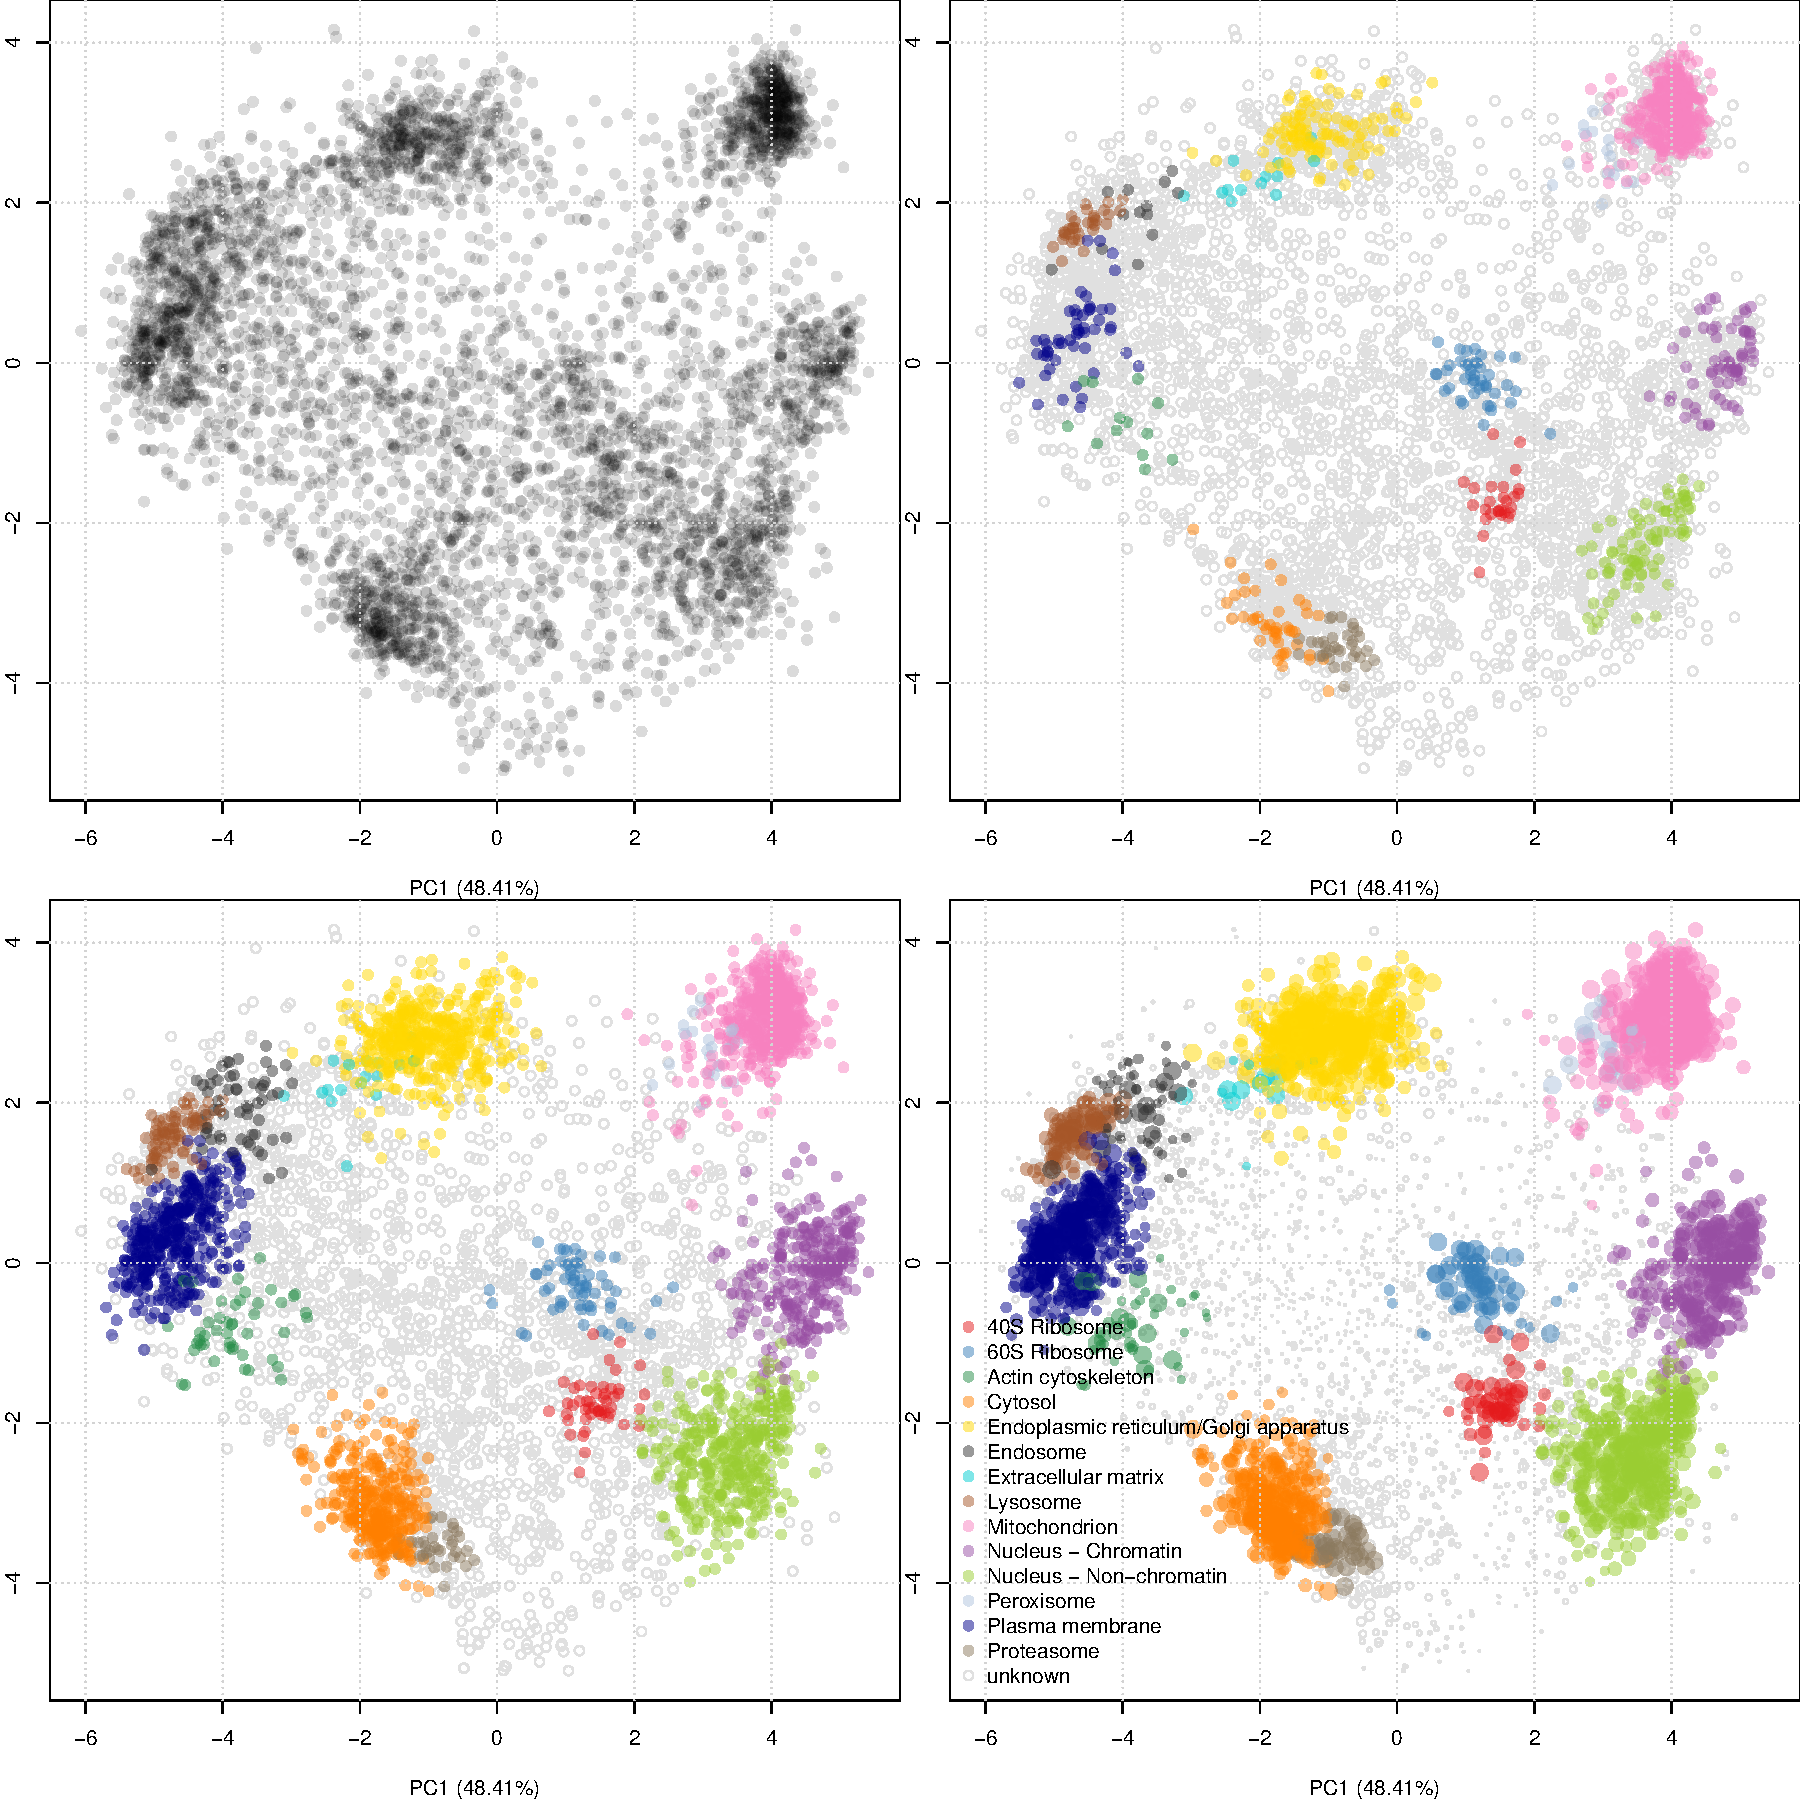
\includegraphics[width=.8\linewidth]{figure/spatprot1eval-1} 

\end{knitrout}
\end{frame}

\begin{frame}[fragile]
  \tiny
\begin{knitrout}
\definecolor{shadecolor}{rgb}{0.969, 0.969, 0.969}\color{fgcolor}\begin{kframe}
\begin{alltt}
\hlkwd{unknownMSnSet}\hlstd{(hyperLOPIT2015)} \hlopt
    \hlstd{fData} \hlopt \hlkwd{select}\hlstd{(final.assignment)} \hlopt \hlstd{table}
\end{alltt}
\begin{verbatim}
## .
##                          40S Ribosome 
##                                    21 
##                          60S Ribosome 
##                                    19 
##                    Actin cytoskeleton 
##                                    33 
##                               Cytosol 
##                                   296 
## Endoplasmic reticulum/Golgi apparatus 
##                                   319 
##                              Endosome 
##                                    47 
##                  Extracellular matrix 
##                                     4 
##                              Lysosome 
##                                    47 
##                         Mitochondrion 
##                                   202 
##                   Nucleus - Chromatin 
##                                   233 
##               Nucleus - Non-chromatin 
##                                   311 
##                            Peroxisome 
##                                     8 
##                       Plasma membrane 
##                                   341 
##                               unknown 
##                                  2225
\end{verbatim}
\end{kframe}
\end{knitrout}
\end{frame}

\begin{frame}[fragile]
    \tiny
\begin{knitrout}
\definecolor{shadecolor}{rgb}{0.969, 0.969, 0.969}\color{fgcolor}\begin{kframe}
\begin{alltt}
\hlkwd{unknownMSnSet}\hlstd{(hyperLOPIT2015)} \hlopt \hlstd{fData} \hlopt
    \hlkwd{select}\hlstd{(final.assignment, svm.score)} \hlopt
    \hlkwd{ggplot}\hlstd{(}\hlkwd{aes}\hlstd{(}\hlkwc{x} \hlstd{= final.assignment,} \hlkwc{y} \hlstd{= svm.score))} \hlopt{+}
    \hlkwd{geom_boxplot}\hlstd{(}\hlkwd{aes}\hlstd{(}\hlkwc{fill} \hlstd{=  final.assignment))}
\end{alltt}
\end{kframe}
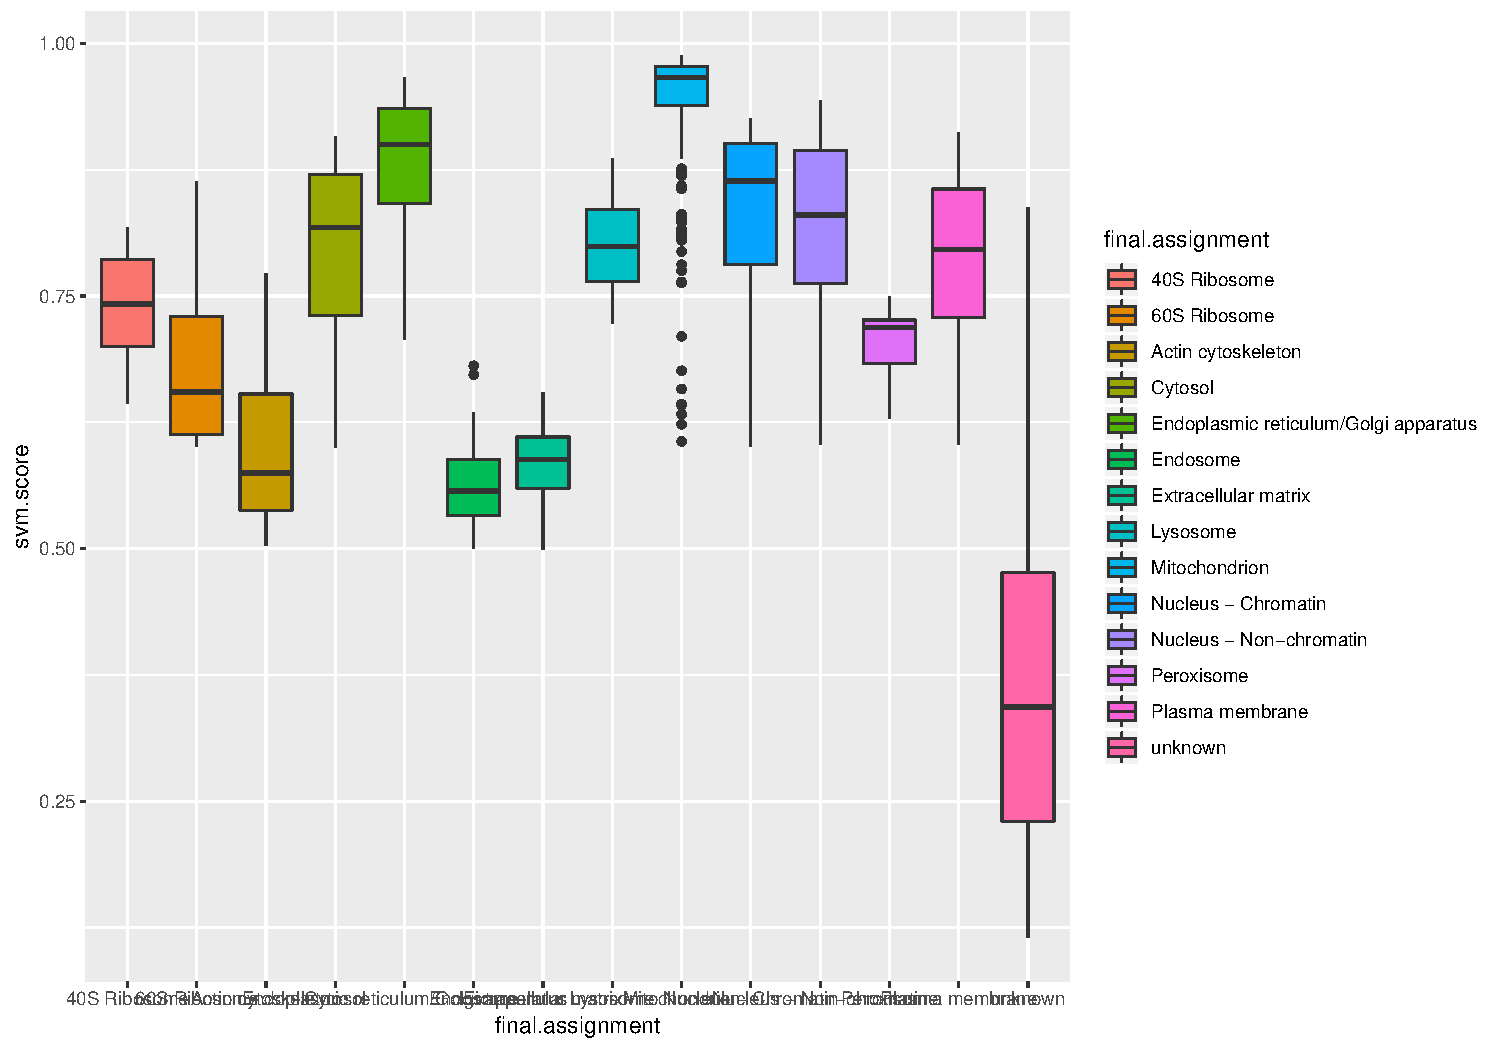
\includegraphics[width=\maxwidth]{figure/spatprot3-1} 

\end{knitrout}
\end{frame}
